% !TeX root = ../main.tex
% !TeX spellcheck = sk_SK
% !TeX encoding = UTF-8
\chapter{Základné pojmy}
V kapitole sú popísané základné pojmy. 

\section{Systémy \acs{SCADA} / HMI}

Vizualizačné systémy sú stystémy realizajúce vizualizáciu procesov. Supervisory Control and Data Acquisition / Human Machine Interface - je Supervízorové riadenie a zber údajov / Rozhranie človek stroj. 
Prenáša informáciu od stroja k ľuďom, čo umožňuje riadenie, monitorovanie a zaznamenávanie systému cez interfejs ako obrázok, klávesnicu, ethernet, touchscree, softvér atď. 


\section{\acs{HTML}5 štandard}

\ac{W3C} vydalo štandard \acs{HTML}5 dňa 28. októbra 2014. 
HTML5 je podporovaný vo všetkých moderných webových prehliadačoch. 
Na obrázku \ref{fig:obrazokHTML} je HTML5 \acs{API} a súvisiace taxonómia technológií a ich status. 

\begin{center}
	\begin{figure}[H]
\centering
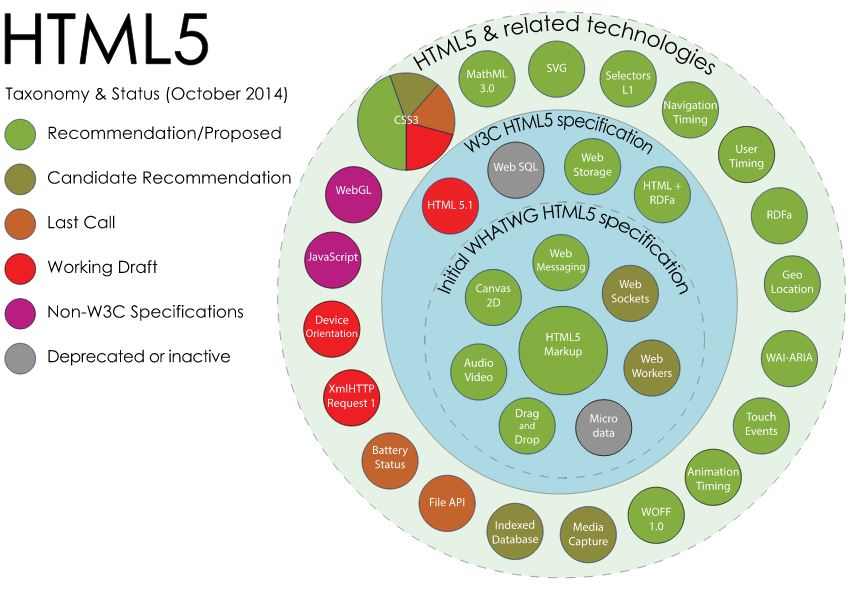
\includegraphics[width=0.7\linewidth]{obrazky/obrazokHTML}
\caption{HTML 5 API}
\label{fig:obrazokHTML}
\end{figure}
\end{center}

HTML5 Graphics definuje dva spôsoby vykreslenia využívajúc: 
\begin{itemize}
	\item $<$canvas$>$ - JavaScript
	\item $<$svg$>$ - SVG
\end{itemize}


\section{Čo je SVG?}
\ac{SVG} je štandardný formát pre vektorovú grafiku. Vektorová grafika je definovaná cez body, priamky, mnohouholníky, elipsy, krivky, alebo iné geometrické tvary.  

\acs{SVG} je jazyk na opísanie dvojrozmernej grafiky v   \ac*{XML}. Vďaka tomu, umožňuje reprezentáciu grafických informácii v kompaktnom a prenositeľnom tvare.

 SVG povoľuje tieto tri typy grafických objektov: vektorové grafické tvary, obrázky a text. 
Grafické objekty môžu byť zoskupené, štylizované, zmenené, a kombinované do predošlých vrstiev objektov. 

SVG obrázky môžu byť dynamické a interaktívne.

Prispôsobiteľnosť SVG umožňuje zmeniť veľkosť grafického komponentu bez straty kvality vzhľadu. Čo umožňuje zobraziť responzívne na viacerých možných zariadení. 
SVG sa bude zobrazovať rovnako na rôznych platformách. Je kompatibilná s štandardmi \acs{HTML}5, ktoré navrhla \ac*{W3C}. 


 \subsection{Podpora v webovom prehliadači}
 Súčasné prehliadače plne podporujú $<$svg$>$ elementy.  
  Čísla v tabuľke \ref{svgpreh} špecifikujú prvé verzie webových prehliadačov, ktoré sú schopné zobraziť $<$svg$>$ element.\cite{w3svg}
  
\begin{table}[H]
\begin{center}
		\begin{tabular}{|c|c|c|c|c|c|}
		\hline \textbf{Element} & \textbf{Chrome} & \textbf{Internet} \textbf{Explorer}  & \textbf{Firefox}  & \textbf{Safari} & \textbf{Opera}  \\ 
		\hline $<svg>$ & 4.0& 9.0 & 3.0 & 3.2  &   10.1 \\ 
		\hline 
	\end{tabular} 
\end{center}
	
	\caption{Podpora HTML $<svg>$ elementu v webových prehliadačoch}
	\label{svgpreh}
\end{table}
 
 \begin{figure}[H]
\centering
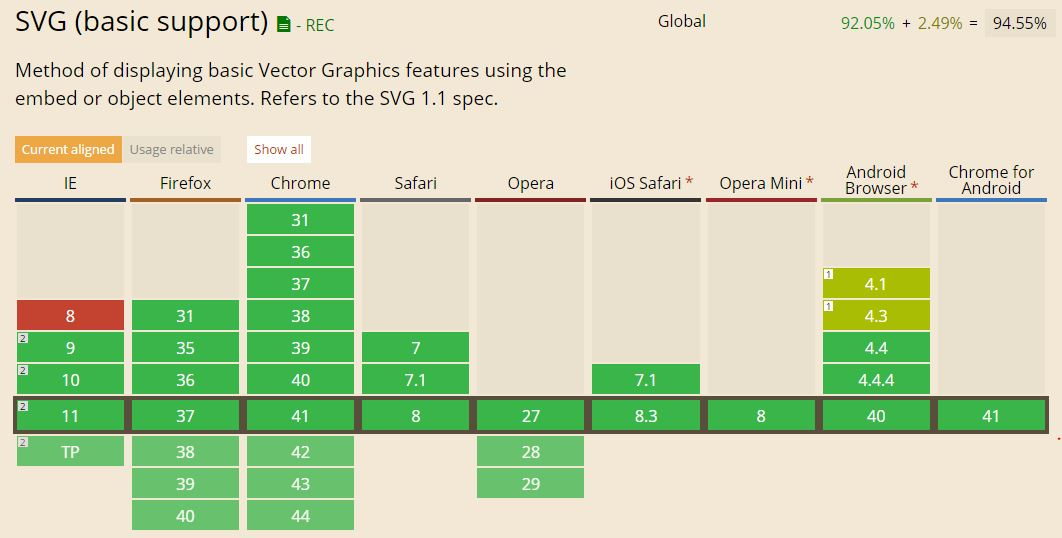
\includegraphics[width=0.7\linewidth]{obrazky/podpora}
\caption{Podpora SVG vo webových prehliadačoch}
\label{fig:podpora}
\end{figure}
% http://caniuse.com/#feat=svg
 
 \subsection{Rozdiely medzi SVG a Canvas}
 %\url{http://www.petrpexa.cz/diplomky/trantyr.pdf} strana 52

SVG patrí do vektorovej grafiky a Canvas zase do raster bitmap grafiky. 
 SVG je jazyk na opísanie dvojrozmernej grafiky v XML.  Canvas kreslí dvojrozmernú grafiku za behu programu cez JavaScript.  SVG je XML založený, čo znamená, že každý element je dostupný cez SVG DOM.   JavaScript umožňuje ovládanie udalostí elementov. V SVG je každý tvar zapamätaný ako objekt.  V prípade zmeny $<$svg$>$ elementu sa automaticky prekreslí.  
 
 
 Canvas je prekresľovaný pixel za pixelom. Bitmapová grafika je zložitejšia pre dynamické prekresľovanie, a má menšie pamäťové nároky a je rýchlejšie. 

Zariadenia ako moderné smartfóny majú veľmi vysokú hustotu pixelov. Niektoré potĺáčajú 300 \ac{PPI} s tým, že sa spoliehajú na obmedzenosť ľudských očí rozoznávať jemné detaily. Pixel nemá v reálnom živote equivalent vo veľkosti až pokým je na obrazovke s fixovaným rozmerom a rozlíšením. Text s veľkosťou 16 pixelov bude veľmi malý pre oko. Pre tento dôvod zariadenia jednoducho nezobrazujú 1 CSS pixelovú jednotku na 1 pixel zariadenia. Namiesto toho zdvoja svoju veľkosť.  
%http://www.smashingmagazine.com/2012/01/16/resolution-independence-with-svg/

%SVG and relative sizes, we have solved the three big issues highlighted above. A scalable graphic can be rasterized on demand to perfectly suit any device resolution and any zoom level. By using relative sizes, we can continue implementing a responsive design, minimizing as much as possible the need for the user to zoom. We’re also respecting the browser’s default font size, and enabling our design to adapt accordingly.


 Tabuľka \ref{canvas:SVG} zobrazuje niekoľko dôležitých odlišností medzi Canvas a SVG. 
% The table below shows some important differences between Canvas and SVG:

 \begin{table}[H]
 \centering
 \begin{tabular}{|l|p{7.5cm} |}
 	\hline \textbf{Canvas} & \textbf{SVG} \\
 	 	\hline Závislé na rozlíšení a \acs{DPI} & Nezávislé na rozlíšení a DPI \\ 
 	\hline Nepodporuje dynamické zmeny & Podporuje dynamické zmeny \\ 
 	\hline Obmedzené možnosti na vykresľovanie  & Vhodné pre aplikácie s veľkými plochami na vykresľovanie \\ 
 	\hline & Väčší výpočtový výkon pri komplexnom obrázku \\ 
 	\hline Vhodné pre grafické-intenzívne hry & Nevhodné pre dynamické hry \\ 
 	\hline 
 \end{tabular} 

 \caption{Porovnanie Canvas a SVG}
 \label{canvas:SVG}
 
\end{table}
 
 
% \section{\acs*{SVG} v HTML dokumente}
%
%SVG môže byť zobrazená buď ako inline v HTML dokumente, alebo ako vloženým samostatného .SVG súboru. 
%V tabuľke \ref{vytvorenie:SVG} sú vymenované HTML tagy na zobrazenie SVG. 
%
%
%
%\begin{table}[hp]
%	\begin{center}
%		\begin{tabular}{|l|l|}
%			\hline \textbf{Technika} & \textbf{Popis} \\ 
%			\hline $<$embed$>$ tag & Načíta vytvorený SVG súbor.  \\ 
%			\hline $<$object$>$ tag & Nepovoľuje skriptovanie.  \\ 
%			\hline $<$iframe$>$ tag & Zobrazí SVG v rámci  \\ 
%			\hline Inline & Vytvorí Svg súbor \\ 
%			\hline
%		\end{tabular} 
%	\end{center}
%	\caption{Spôsoby vytvorenia SVG v HTML dokumente}
%	\label{vytvorenie:SVG}
%\end{table}
%
%\subsection{Príklady načítania SVG v HTML dokumente}
%
%	\subsubsection{Image}
%	\begin{lstlisting}
%<img src="stanica2.svg" width = "50" height= "50" />
%	\end{lstlisting}
%	
%	\subsubsection{Embed}
%	\begin{lstlisting}
%<embed src="stanica2.svg" width = "50" height= "50" />
%	\end{lstlisting}
%	
%	
%\subsubsection{Object}
%
%	\begin{lstlisting}
%<object type="image/svg+xml" data="stanica2.svg"
%	width="50" height="50"></object>
%	\end{lstlisting}
%	
%	
%\subsubsection{	Iframe}
%
%	\begin{lstlisting}
%<iframe src="stanica2.svg" width = "50" height= "50"><</iframe>
%	\end{lstlisting}







%\subsection{Príklad použitia SVG v HTML dokumente s inline SVG}
%
%HTML kód: 
%
%\begin{lstlisting}
%<!DOCTYPE html>
%<html>
%<head lang="sk">
%	<meta charset="UTF-8">
%	<title>Bakalarska praca</title>
%</head> <body>
%	<svg width="100" height="100">
%		<circle cx="50" cy="50" r="40" stroke="black" stroke-width="2" fill="silver" />
%	</svg>	
%</body>
%</html>
%
%\end{lstlisting}
%
%SVG obrázok začína s $<$svg$>$ elementom. Atribúty elementu $<$svg$>$ sú width a height. Definujú šírku a výšku SVG obrázka. Element $<$circle$>$ je použitý na nakreslenie kruhu.
%
% Atribúty cx, cy definujú x, y súradnice od centra kruhu. Ak je cx, cy vynechané, tak center kruhu je nastavený na $($0, 0$)$. Atribút r  definuje polomer kruhu. Atribúty stroke a stroke-width určujú to ako bude vyzerať obrys útvaru. Kruh má nastavený 2px čierny okraj. 
%Atribút fill vyplní vnútro kruhu. V príklade je vyplnený sivou farbou. Tag, ktorý uzavrie SVG obrázok je $<$$/$svg$>$. Keďže SVG je validné XML, tak všetky elementy musia byť správne zatvorené. \cite{inline} Vykreslí na HTML webovú stránku útvar, ktorý je na obrázku \ref{jednoduchyKruh}.
%
%\begin{figure}[hp]
%	\begin{center}
%		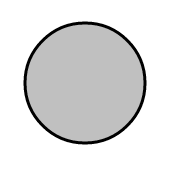
\includegraphics  {obrazky/jednoduchyKruh.png}
%		\caption{Vykreslenie SVG na HTML stránke}
%		\label{jednoduchyKruh}
%	\end{center}
%\end{figure}


%\section{SVG tvary} 
%
%\acs*{SVG} má preddefinované tvary elementov:
%\begin{itemize}
%	\item Obdĺžník $<$rect$>$
%	\item Kruh $<$circle$>$
%	\item Elipsa $<$ellipse$>$
%	\item Čiara $<$line$>$
%	\item Polyline $<$polyline$>$
%	\item Mnohouholník $<$polygon$>$
%	\item Path $<$path$>$	
%\end{itemize}
%
%Spoločné vlastnosti pre kruh, elipsu, a čiaru sú r, x, y, cx, cy, rx, ry. Teda polomer, pravá a ľavá pozícia,x a y súradnice od stredu, a horizontálny a vertikálny polomer. 
%
%\subsection{Element Path} 
%
%TODO NIECO NAPISAT K TOMU
%
%\begin{center}
%	\begin{table}
%		\begin{center}
%			\begin{tabular}{|c|l|c|}
%				\hline \textbf{Príkaz} & \textbf{Názov} & \textbf{Parametre} \\
%				\hline M & moveto & (x y)+ \\ 
%				\hline Z & closepath & (none) \\ 
%				\hline L & lineto & (x y)+ \\ 
%				\hline H & horizonal lineto & x+ \\ 
%				\hline V & vertical lineto & y+ \\ 
%				\hline C & curveto & (x1 y1 x2 y2 x y)+ \\ 
%				\hline S & smooth curveto & (x2 y2 x y)+ \\ 
%				\hline Q & quadratic Bézier curveto & (x1 y1 x y)+ \\ 
%				\hline T & smooth quadratic Bézier curveto & (x y)+ \\ 
%				\hline 
%			\end{tabular} 
%		\end{center}
%		\caption{Niekoľko príkazov na tvorbu Path elementu}
%		\label{prikazyPath}
%	\end{table}
%\end{center}

%https://msdn.microsoft.com/en-us/hh552482.aspx